\documentclass{standalone}
\usepackage{tikz}
\usetikzlibrary{patterns, positioning}


\begin{document}
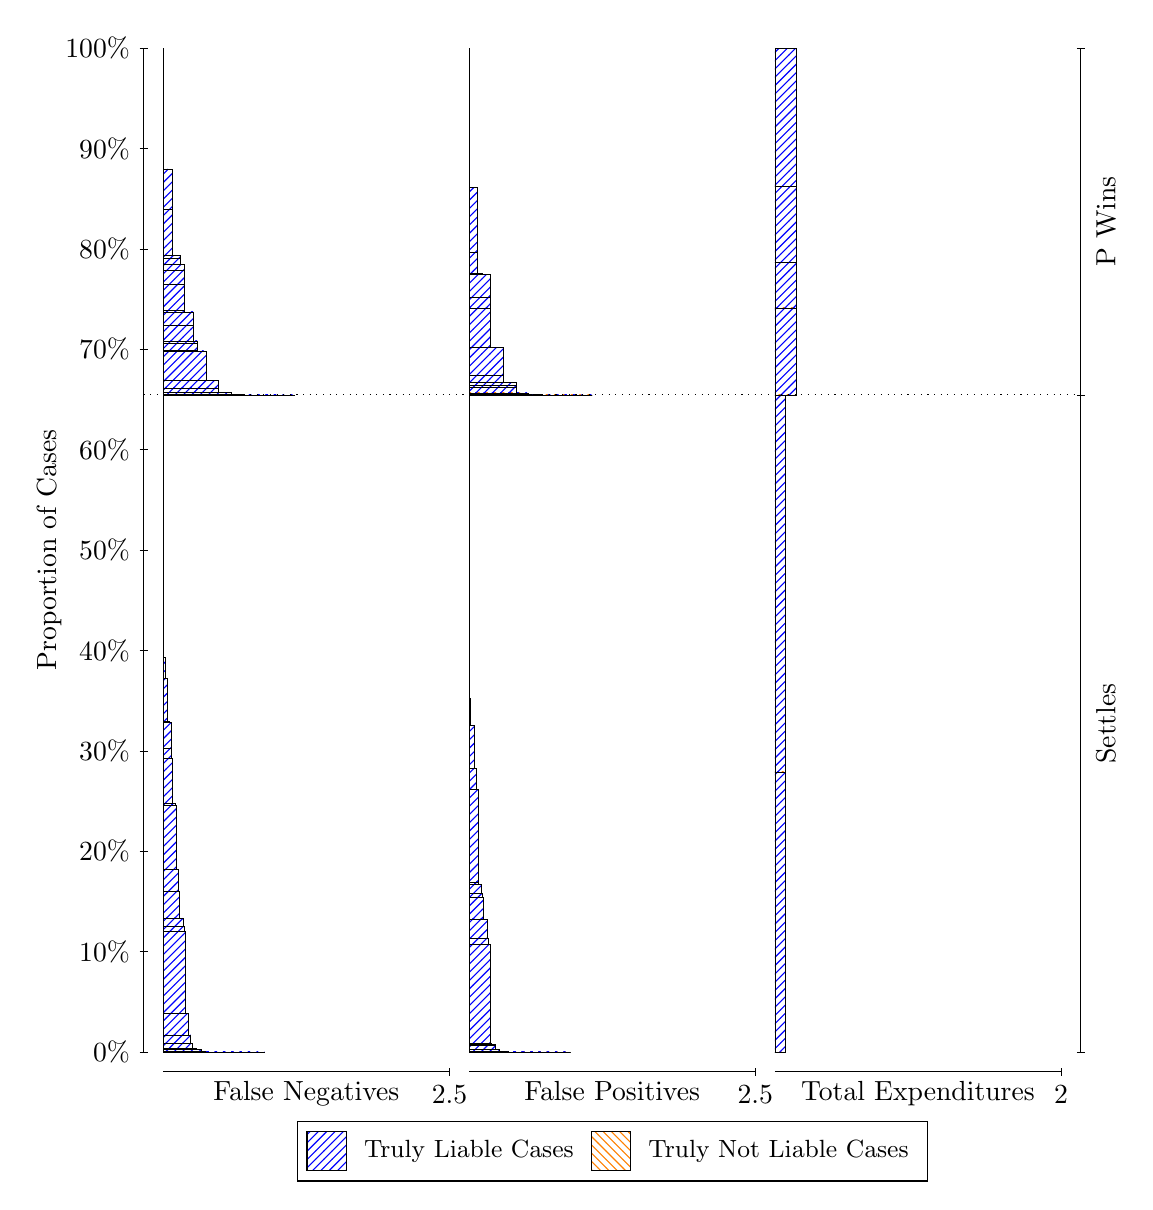
\begin{tikzpicture}
\draw[black, very thin] (1.5,1.75) -- (1.5,14.5);
\node[rotate=90, text=black, anchor=center] at (0.3, 8.125) {Proportion of Cases};
\draw[black, very thin] (1.45,1.75) -- (1.55,1.75);
\node[text=black, anchor=east] at (1.45, 1.75) {0\%};
\draw[black, very thin] (1.45,3.025) -- (1.55,3.025);
\node[text=black, anchor=east] at (1.45, 3.025) {10\%};
\draw[black, very thin] (1.45,4.3) -- (1.55,4.3);
\node[text=black, anchor=east] at (1.45, 4.3) {20\%};
\draw[black, very thin] (1.45,5.575) -- (1.55,5.575);
\node[text=black, anchor=east] at (1.45, 5.575) {30\%};
\draw[black, very thin] (1.45,6.85) -- (1.55,6.85);
\node[text=black, anchor=east] at (1.45, 6.85) {40\%};
\draw[black, very thin] (1.45,8.125) -- (1.55,8.125);
\node[text=black, anchor=east] at (1.45, 8.125) {50\%};
\draw[black, very thin] (1.45,9.4) -- (1.55,9.4);
\node[text=black, anchor=east] at (1.45, 9.4) {60\%};
\draw[black, very thin] (1.45,10.675) -- (1.55,10.675);
\node[text=black, anchor=east] at (1.45, 10.675) {70\%};
\draw[black, very thin] (1.45,11.95) -- (1.55,11.95);
\node[text=black, anchor=east] at (1.45, 11.95) {80\%};
\draw[black, very thin] (1.45,13.225) -- (1.55,13.225);
\node[text=black, anchor=east] at (1.45, 13.225) {90\%};
\draw[black, very thin] (1.45,14.5) -- (1.55,14.5);
\node[text=black, anchor=east] at (1.45, 14.5) {100\%};

\draw[black, very thin] (13.4,1.75) -- (13.4,14.5);
\draw[black, very thin] (13.35,1.75) -- (13.45,1.75);
\node[anchor=west] at (13.35, 1.75) {};
\draw[black, very thin] (13.35,10.095) -- (13.45,10.095);
\node[anchor=west] at (13.35, 10.095) {};
\draw[black, very thin] (13.35,14.5) -- (13.45,14.5);
\node[anchor=west] at (13.35, 14.5) {};

\draw[black, very thin, pattern color=blue, pattern=north east lines] (1.75,1.75) rectangle (3.0398,1.75);
\draw[black, very thin, pattern color=blue, pattern=north east lines] (1.75,1.75) rectangle (2.8784,1.75);
\draw[black, very thin, pattern color=blue, pattern=north east lines] (1.75,1.75) rectangle (2.8218,1.75);
\draw[black, very thin, pattern color=blue, pattern=north east lines] (1.75,1.75) rectangle (2.7169,1.75);
\draw[black, very thin, pattern color=blue, pattern=north east lines] (1.75,1.75) rectangle (2.6604,1.75);
\draw[black, very thin, pattern color=blue, pattern=north east lines] (1.75,1.75) rectangle (2.6038,1.75);
\draw[black, very thin, pattern color=blue, pattern=north east lines] (1.75,1.75) rectangle (2.5554,1.75);
\draw[black, very thin, pattern color=blue, pattern=north east lines] (1.75,1.75) rectangle (2.5312,1.75);
\draw[black, very thin, pattern color=blue, pattern=north east lines] (1.75,1.75) rectangle (2.4989,1.75);
\draw[black, very thin, pattern color=blue, pattern=north east lines] (1.75,1.75) rectangle (2.4424,1.75);
\draw[black, very thin, pattern color=blue, pattern=north east lines] (1.75,1.75) rectangle (2.3939,1.7506);
\draw[black, very thin, pattern color=blue, pattern=north east lines] (1.75,1.7506) rectangle (2.3858,1.7506);
\draw[black, very thin, pattern color=blue, pattern=north east lines] (1.75,1.7506) rectangle (2.3697,1.7506);
\draw[black, very thin, pattern color=blue, pattern=north east lines] (1.75,1.7506) rectangle (2.3374,1.7508);
\draw[black, very thin, pattern color=blue, pattern=north east lines] (1.75,1.7508) rectangle (2.3132,1.7508);
\draw[black, very thin, pattern color=blue, pattern=north east lines] (1.75,1.7508) rectangle (2.2809,1.7532);
\draw[black, very thin, pattern color=blue, pattern=north east lines] (1.75,1.7532) rectangle (2.2324,1.7795);
\draw[black, very thin, pattern color=blue, pattern=north east lines] (1.75,1.7795) rectangle (2.2244,1.7796);
\draw[black, very thin, pattern color=blue, pattern=north east lines] (1.75,1.7796) rectangle (2.2082,1.7796);
\draw[black, very thin, pattern color=blue, pattern=north east lines] (1.75,1.7796) rectangle (2.1759,1.7865);
\draw[black, very thin, pattern color=blue, pattern=north east lines] (1.75,1.7865) rectangle (2.1678,1.7973);
\draw[black, very thin, pattern color=blue, pattern=north east lines] (1.75,1.7973) rectangle (2.1517,1.7975);
\draw[black, very thin, pattern color=blue, pattern=north east lines] (1.75,1.7975) rectangle (2.1194,1.8557);
\draw[black, very thin, pattern color=blue, pattern=north east lines] (1.75,1.8557) rectangle (2.0952,1.967);
\draw[black, very thin, pattern color=blue, pattern=north east lines] (1.75,1.967) rectangle (2.0709,2.2389);
\draw[black, very thin, pattern color=blue, pattern=north east lines] (1.75,2.2389) rectangle (2.0629,2.2419);
\draw[black, very thin, pattern color=blue, pattern=north east lines] (1.75,2.2419) rectangle (2.0467,2.242);
\draw[black, very thin, pattern color=blue, pattern=north east lines] (1.75,2.242) rectangle (2.0225,3.2825);
\draw[black, very thin, pattern color=blue, pattern=north east lines] (1.75,3.2825) rectangle (2.0144,3.3409);
\draw[black, very thin, pattern color=blue, pattern=north east lines] (1.75,3.3409) rectangle (2.0064,3.45);
\draw[black, very thin, pattern color=blue, pattern=north east lines] (1.75,3.45) rectangle (1.9902,3.4524);
\draw[black, very thin, pattern color=blue, pattern=north east lines] (1.75,3.4524) rectangle (1.9579,3.7868);
\draw[black, very thin, pattern color=blue, pattern=north east lines] (1.75,3.7868) rectangle (1.9337,4.0688);
\draw[black, very thin, pattern color=blue, pattern=north east lines] (1.75,4.0688) rectangle (1.9095,4.8889);
\draw[black, very thin, pattern color=blue, pattern=north east lines] (1.75,4.8889) rectangle (1.9014,4.9094);
\draw[black, very thin, pattern color=blue, pattern=north east lines] (1.75,4.9094) rectangle (1.8852,4.9094);
\draw[black, very thin, pattern color=blue, pattern=north east lines] (1.75,4.9094) rectangle (1.861,5.4807);
\draw[black, very thin, pattern color=blue, pattern=north east lines] (1.75,5.4807) rectangle (1.8529,5.602);
\draw[black, very thin, pattern color=blue, pattern=north east lines] (1.75,5.602) rectangle (1.8449,5.9407);
\draw[black, very thin, pattern color=blue, pattern=north east lines] (1.75,5.9407) rectangle (1.8287,5.9464);
\draw[black, very thin, pattern color=blue, pattern=north east lines] (1.75,5.9464) rectangle (1.7964,6.4927);
\draw[black, very thin, pattern color=blue, pattern=north east lines] (1.75,6.4927) rectangle (1.7722,6.7601);
\draw[black, very thin, pattern color=orange, pattern=north west lines] (1.75,6.7601) rectangle (1.75,6.7601);
\draw[black, very thin, pattern color=blue, pattern=north east lines] (1.75,6.7601) rectangle (1.75,10.095);
\draw[black, very thin, pattern color=blue, pattern=north east lines] (1.75,10.095) rectangle (3.4213,10.095);
\draw[black, very thin, pattern color=blue, pattern=north east lines] (1.75,10.095) rectangle (3.2599,10.095);
\draw[black, very thin, pattern color=blue, pattern=north east lines] (1.75,10.095) rectangle (3.2599,10.095);
\draw[black, very thin, pattern color=blue, pattern=north east lines] (1.75,10.095) rectangle (3.0984,10.095);
\draw[black, very thin, pattern color=blue, pattern=north east lines] (1.75,10.095) rectangle (3.0984,10.095);
\draw[black, very thin, pattern color=blue, pattern=north east lines] (1.75,10.095) rectangle (2.9894,10.095);
\draw[black, very thin, pattern color=blue, pattern=north east lines] (1.75,10.095) rectangle (2.9369,10.095);
\draw[black, very thin, pattern color=blue, pattern=north east lines] (1.75,10.095) rectangle (2.8279,10.095);
\draw[black, very thin, pattern color=blue, pattern=north east lines] (1.75,10.095) rectangle (2.7754,10.097);
\draw[black, very thin, pattern color=blue, pattern=north east lines] (1.75,10.097) rectangle (2.7754,10.099);
\draw[black, very thin, pattern color=blue, pattern=north east lines] (1.75,10.099) rectangle (2.6664,10.099);
\draw[black, very thin, pattern color=blue, pattern=north east lines] (1.75,10.099) rectangle (2.6139,10.128);
\draw[black, very thin, pattern color=blue, pattern=north east lines] (1.75,10.128) rectangle (2.5049,10.128);
\draw[black, very thin, pattern color=blue, pattern=north east lines] (1.75,10.128) rectangle (2.5049,10.128);
\draw[black, very thin, pattern color=blue, pattern=north east lines] (1.75,10.128) rectangle (2.4524,10.185);
\draw[black, very thin, pattern color=blue, pattern=north east lines] (1.75,10.185) rectangle (2.4524,10.275);
\draw[black, very thin, pattern color=blue, pattern=north east lines] (1.75,10.275) rectangle (2.3434,10.279);
\draw[black, very thin, pattern color=blue, pattern=north east lines] (1.75,10.279) rectangle (2.3434,10.28);
\draw[black, very thin, pattern color=blue, pattern=north east lines] (1.75,10.28) rectangle (2.3434,10.284);
\draw[black, very thin, pattern color=blue, pattern=north east lines] (1.75,10.284) rectangle (2.291,10.653);
\draw[black, very thin, pattern color=blue, pattern=north east lines] (1.75,10.653) rectangle (2.182,10.662);
\draw[black, very thin, pattern color=blue, pattern=north east lines] (1.75,10.662) rectangle (2.182,10.75);
\draw[black, very thin, pattern color=blue, pattern=north east lines] (1.75,10.75) rectangle (2.182,10.782);
\draw[black, very thin, pattern color=blue, pattern=north east lines] (1.75,10.782) rectangle (2.1295,10.976);
\draw[black, very thin, pattern color=blue, pattern=north east lines] (1.75,10.976) rectangle (2.1295,11.148);
\draw[black, very thin, pattern color=blue, pattern=north east lines] (1.75,11.148) rectangle (2.0205,11.165);
\draw[black, very thin, pattern color=blue, pattern=north east lines] (1.75,11.165) rectangle (2.0205,11.497);
\draw[black, very thin, pattern color=blue, pattern=north east lines] (1.75,11.497) rectangle (2.0205,11.673);
\draw[black, very thin, pattern color=blue, pattern=north east lines] (1.75,11.673) rectangle (2.0205,11.751);
\draw[black, very thin, pattern color=blue, pattern=north east lines] (1.75,11.751) rectangle (1.968,11.827);
\draw[black, very thin, pattern color=blue, pattern=north east lines] (1.75,11.827) rectangle (1.968,11.867);
\draw[black, very thin, pattern color=blue, pattern=north east lines] (1.75,11.867) rectangle (1.859,12.447);
\draw[black, very thin, pattern color=blue, pattern=north east lines] (1.75,12.447) rectangle (1.859,12.956);
\draw[black, very thin, pattern color=blue, pattern=north east lines] (1.75,12.956) rectangle (1.8065,12.956);
\draw[black, very thin, pattern color=blue, pattern=north east lines] (1.75,12.956) rectangle (1.8065,12.962);
\draw[black, very thin, pattern color=blue, pattern=north east lines] (1.75,12.962) rectangle (1.8065,12.966);
\draw[black, very thin, pattern color=blue, pattern=north east lines] (1.75,12.966) rectangle (1.8065,12.966);
\draw[black, very thin, pattern color=orange, pattern=north west lines] (1.75,12.966) rectangle (1.75,12.966);
\draw[black, very thin, pattern color=blue, pattern=north east lines] (1.75,12.966) rectangle (1.75,14.5);
\draw[black, very thin, pattern color=orange, pattern=north west lines] (5.6333,1.75) rectangle (6.9232,1.75);
\draw[black, very thin, pattern color=blue, pattern=north east lines] (5.6333,1.75) rectangle (6.9232,1.75);
\draw[black, very thin, pattern color=orange, pattern=north west lines] (5.6333,1.75) rectangle (6.8505,1.75);
\draw[black, very thin, pattern color=blue, pattern=north east lines] (5.6333,1.75) rectangle (6.8505,1.75);
\draw[black, very thin, pattern color=orange, pattern=north west lines] (5.6333,1.75) rectangle (6.7778,1.75);
\draw[black, very thin, pattern color=blue, pattern=north east lines] (5.6333,1.75) rectangle (6.7778,1.75);
\draw[black, very thin, pattern color=blue, pattern=north east lines] (5.6333,1.75) rectangle (6.7617,1.75);
\draw[black, very thin, pattern color=blue, pattern=north east lines] (5.6333,1.75) rectangle (6.689,1.75);
\draw[black, very thin, pattern color=orange, pattern=north west lines] (5.6333,1.75) rectangle (6.6325,1.75);
\draw[black, very thin, pattern color=blue, pattern=north east lines] (5.6333,1.75) rectangle (6.6325,1.75);
\draw[black, very thin, pattern color=blue, pattern=north east lines] (5.6333,1.75) rectangle (6.6164,1.75);
\draw[black, very thin, pattern color=blue, pattern=north east lines] (5.6333,1.75) rectangle (6.6002,1.75);
\draw[black, very thin, pattern color=orange, pattern=north west lines] (5.6333,1.75) rectangle (6.5598,1.75);
\draw[black, very thin, pattern color=blue, pattern=north east lines] (5.6333,1.75) rectangle (6.5598,1.75);
\draw[black, very thin, pattern color=blue, pattern=north east lines] (5.6333,1.75) rectangle (6.5275,1.75);
\draw[black, very thin, pattern color=blue, pattern=north east lines] (5.6333,1.75) rectangle (6.471,1.75);
\draw[black, very thin, pattern color=blue, pattern=north east lines] (5.6333,1.75) rectangle (6.4549,1.75);
\draw[black, very thin, pattern color=blue, pattern=north east lines] (5.6333,1.75) rectangle (6.4387,1.75);
\draw[black, very thin, pattern color=orange, pattern=north west lines] (5.6333,1.75) rectangle (6.4145,1.75);
\draw[black, very thin, pattern color=blue, pattern=north east lines] (5.6333,1.75) rectangle (6.4145,1.75);
\draw[black, very thin, pattern color=blue, pattern=north east lines] (5.6333,1.75) rectangle (6.3984,1.75);
\draw[black, very thin, pattern color=blue, pattern=north east lines] (5.6333,1.75) rectangle (6.3661,1.75);
\draw[black, very thin, pattern color=orange, pattern=north west lines] (5.6333,1.75) rectangle (6.3418,1.75);
\draw[black, very thin, pattern color=blue, pattern=north east lines] (5.6333,1.75) rectangle (6.3418,1.75);
\draw[black, very thin, pattern color=blue, pattern=north east lines] (5.6333,1.75) rectangle (6.3095,1.75);
\draw[black, very thin, pattern color=blue, pattern=north east lines] (5.6333,1.75) rectangle (6.2934,1.75);
\draw[black, very thin, pattern color=blue, pattern=north east lines] (5.6333,1.75) rectangle (6.2772,1.75);
\draw[black, very thin, pattern color=blue, pattern=north east lines] (5.6333,1.75) rectangle (6.253,1.75);
\draw[black, very thin, pattern color=blue, pattern=north east lines] (5.6333,1.75) rectangle (6.2369,1.75);
\draw[black, very thin, pattern color=blue, pattern=north east lines] (5.6333,1.75) rectangle (6.2046,1.7501);
\draw[black, very thin, pattern color=blue, pattern=north east lines] (5.6333,1.7501) rectangle (6.1804,1.7507);
\draw[black, very thin, pattern color=blue, pattern=north east lines] (5.6333,1.7507) rectangle (6.1481,1.7507);
\draw[black, very thin, pattern color=blue, pattern=north east lines] (5.6333,1.7507) rectangle (6.1319,1.7531);
\draw[black, very thin, pattern color=orange, pattern=north west lines] (5.6333,1.7531) rectangle (6.1238,1.7531);
\draw[black, very thin, pattern color=blue, pattern=north east lines] (5.6333,1.7531) rectangle (6.1238,1.7535);
\draw[black, very thin, pattern color=blue, pattern=north east lines] (5.6333,1.7535) rectangle (6.1158,1.7535);
\draw[black, very thin, pattern color=blue, pattern=north east lines] (5.6333,1.7535) rectangle (6.0915,1.7535);
\draw[black, very thin, pattern color=blue, pattern=north east lines] (5.6333,1.7535) rectangle (6.0754,1.7537);
\draw[black, very thin, pattern color=blue, pattern=north east lines] (5.6333,1.7537) rectangle (6.0431,1.7592);
\draw[black, very thin, pattern color=blue, pattern=north east lines] (5.6333,1.7592) rectangle (6.0189,1.7852);
\draw[black, very thin, pattern color=blue, pattern=north east lines] (5.6333,1.7852) rectangle (5.9866,1.7854);
\draw[black, very thin, pattern color=blue, pattern=north east lines] (5.6333,1.7854) rectangle (5.9704,1.8384);
\draw[black, very thin, pattern color=blue, pattern=north east lines] (5.6333,1.8384) rectangle (5.9624,1.8462);
\draw[black, very thin, pattern color=blue, pattern=north east lines] (5.6333,1.8462) rectangle (5.9543,1.8519);
\draw[black, very thin, pattern color=blue, pattern=north east lines] (5.6333,1.8519) rectangle (5.9301,1.8519);
\draw[black, very thin, pattern color=blue, pattern=north east lines] (5.6333,1.8519) rectangle (5.9139,1.8567);
\draw[black, very thin, pattern color=orange, pattern=north west lines] (5.6333,1.8567) rectangle (5.9058,1.8567);
\draw[black, very thin, pattern color=blue, pattern=north east lines] (5.6333,1.8567) rectangle (5.9058,3.1198);
\draw[black, very thin, pattern color=blue, pattern=north east lines] (5.6333,3.1198) rectangle (5.8816,3.1933);
\draw[black, very thin, pattern color=blue, pattern=north east lines] (5.6333,3.1933) rectangle (5.8574,3.4391);
\draw[black, very thin, pattern color=blue, pattern=north east lines] (5.6333,3.4391) rectangle (5.8251,3.4415);
\draw[black, very thin, pattern color=blue, pattern=north east lines] (5.6333,3.4415) rectangle (5.8089,3.7086);
\draw[black, very thin, pattern color=blue, pattern=north east lines] (5.6333,3.7086) rectangle (5.8009,3.7677);
\draw[black, very thin, pattern color=blue, pattern=north east lines] (5.6333,3.7677) rectangle (5.7928,3.8857);
\draw[black, very thin, pattern color=blue, pattern=north east lines] (5.6333,3.8857) rectangle (5.7686,3.8858);
\draw[black, very thin, pattern color=blue, pattern=north east lines] (5.6333,3.8858) rectangle (5.7524,3.9091);
\draw[black, very thin, pattern color=blue, pattern=north east lines] (5.6333,3.9091) rectangle (5.7444,5.085);
\draw[black, very thin, pattern color=blue, pattern=north east lines] (5.6333,5.085) rectangle (5.7201,5.3524);
\draw[black, very thin, pattern color=blue, pattern=north east lines] (5.6333,5.3524) rectangle (5.6959,5.8987);
\draw[black, very thin, pattern color=blue, pattern=north east lines] (5.6333,5.8987) rectangle (5.6636,5.9043);
\draw[black, very thin, pattern color=blue, pattern=north east lines] (5.6333,5.9043) rectangle (5.6475,6.2431);
\draw[black, very thin, pattern color=blue, pattern=north east lines] (5.6333,6.2431) rectangle (5.6394,6.3643);
\draw[black, very thin, pattern color=blue, pattern=north east lines] (5.6333,6.3643) rectangle (5.6333,10.095);
\draw[black, very thin, pattern color=orange, pattern=north west lines] (5.6333,10.095) rectangle (7.1957,10.095);
\draw[black, very thin, pattern color=blue, pattern=north east lines] (5.6333,10.095) rectangle (7.1957,10.095);
\draw[black, very thin, pattern color=orange, pattern=north west lines] (5.6333,10.095) rectangle (7.0342,10.095);
\draw[black, very thin, pattern color=blue, pattern=north east lines] (5.6333,10.095) rectangle (7.0342,10.095);
\draw[black, very thin, pattern color=orange, pattern=north west lines] (5.6333,10.095) rectangle (6.8727,10.095);
\draw[black, very thin, pattern color=blue, pattern=north east lines] (5.6333,10.095) rectangle (6.8727,10.095);
\draw[black, very thin, pattern color=blue, pattern=north east lines] (5.6333,10.095) rectangle (6.8727,10.095);
\draw[black, very thin, pattern color=blue, pattern=north east lines] (5.6333,10.095) rectangle (6.7112,10.095);
\draw[black, very thin, pattern color=orange, pattern=north west lines] (5.6333,10.095) rectangle (6.7112,10.095);
\draw[black, very thin, pattern color=blue, pattern=north east lines] (5.6333,10.095) rectangle (6.7112,10.095);
\draw[black, very thin, pattern color=orange, pattern=north west lines] (5.6333,10.095) rectangle (6.6022,10.095);
\draw[black, very thin, pattern color=blue, pattern=north east lines] (5.6333,10.095) rectangle (6.6022,10.095);
\draw[black, very thin, pattern color=orange, pattern=north west lines] (5.6333,10.095) rectangle (6.5497,10.095);
\draw[black, very thin, pattern color=blue, pattern=north east lines] (5.6333,10.095) rectangle (6.5497,10.097);
\draw[black, very thin, pattern color=orange, pattern=north west lines] (5.6333,10.097) rectangle (6.4407,10.097);
\draw[black, very thin, pattern color=blue, pattern=north east lines] (5.6333,10.097) rectangle (6.4407,10.097);
\draw[black, very thin, pattern color=orange, pattern=north west lines] (5.6333,10.097) rectangle (6.3883,10.097);
\draw[black, very thin, pattern color=blue, pattern=north east lines] (5.6333,10.097) rectangle (6.3883,10.12);
\draw[black, very thin, pattern color=blue, pattern=north east lines] (5.6333,10.12) rectangle (6.2793,10.12);
\draw[black, very thin, pattern color=orange, pattern=north west lines] (5.6333,10.12) rectangle (6.2793,10.12);
\draw[black, very thin, pattern color=blue, pattern=north east lines] (5.6333,10.12) rectangle (6.2793,10.12);
\draw[black, very thin, pattern color=orange, pattern=north west lines] (5.6333,10.12) rectangle (6.2268,10.12);
\draw[black, very thin, pattern color=blue, pattern=north east lines] (5.6333,10.12) rectangle (6.2268,10.192);
\draw[black, very thin, pattern color=blue, pattern=north east lines] (5.6333,10.192) rectangle (6.2268,10.22);
\draw[black, very thin, pattern color=blue, pattern=north east lines] (5.6333,10.22) rectangle (6.2268,10.253);
\draw[black, very thin, pattern color=blue, pattern=north east lines] (5.6333,10.253) rectangle (6.1178,10.253);
\draw[black, very thin, pattern color=orange, pattern=north west lines] (5.6333,10.253) rectangle (6.1178,10.253);
\draw[black, very thin, pattern color=blue, pattern=north east lines] (5.6333,10.253) rectangle (6.1178,10.253);
\draw[black, very thin, pattern color=orange, pattern=north west lines] (5.6333,10.253) rectangle (6.0653,10.253);
\draw[black, very thin, pattern color=blue, pattern=north east lines] (5.6333,10.253) rectangle (6.0653,10.338);
\draw[black, very thin, pattern color=blue, pattern=north east lines] (5.6333,10.338) rectangle (6.0653,10.703);
\draw[black, very thin, pattern color=blue, pattern=north east lines] (5.6333,10.703) rectangle (5.9563,10.703);
\draw[black, very thin, pattern color=orange, pattern=north west lines] (5.6333,10.703) rectangle (5.9563,10.703);
\draw[black, very thin, pattern color=blue, pattern=north east lines] (5.6333,10.703) rectangle (5.9563,10.703);
\draw[black, very thin, pattern color=blue, pattern=north east lines] (5.6333,10.703) rectangle (5.9038,11.2);
\draw[black, very thin, pattern color=blue, pattern=north east lines] (5.6333,11.2) rectangle (5.9038,11.33);
\draw[black, very thin, pattern color=blue, pattern=north east lines] (5.6333,11.33) rectangle (5.9038,11.629);
\draw[black, very thin, pattern color=blue, pattern=north east lines] (5.6333,11.629) rectangle (5.7948,11.629);
\draw[black, very thin, pattern color=orange, pattern=north west lines] (5.6333,11.629) rectangle (5.7948,11.629);
\draw[black, very thin, pattern color=blue, pattern=north east lines] (5.6333,11.629) rectangle (5.7948,11.639);
\draw[black, very thin, pattern color=blue, pattern=north east lines] (5.6333,11.639) rectangle (5.7948,11.639);
\draw[black, very thin, pattern color=blue, pattern=north east lines] (5.6333,11.639) rectangle (5.7423,11.901);
\draw[black, very thin, pattern color=blue, pattern=north east lines] (5.6333,11.901) rectangle (5.7423,12.728);
\draw[black, very thin, pattern color=orange, pattern=north west lines] (5.6333,12.728) rectangle (5.6333,12.728);
\draw[black, very thin, pattern color=blue, pattern=north east lines] (5.6333,12.728) rectangle (5.6333,14.5);
\draw[black, very thin, pattern color=orange, pattern=north west lines] (9.5167,1.75) rectangle (9.6529,1.75);
\draw[black, very thin, pattern color=blue, pattern=north east lines] (9.5167,1.75) rectangle (9.6529,5.3077);
\draw[black, very thin, pattern color=orange, pattern=north west lines] (9.5167,5.3077) rectangle (9.6529,5.3077);
\draw[black, very thin, pattern color=blue, pattern=north east lines] (9.5167,5.3077) rectangle (9.6529,10.095);
\draw[black, very thin, pattern color=orange, pattern=north west lines] (9.5167,10.095) rectangle (9.7892,10.095);
\draw[black, very thin, pattern color=blue, pattern=north east lines] (9.5167,10.095) rectangle (9.7892,11.2);
\draw[black, very thin, pattern color=orange, pattern=north west lines] (9.5167,11.2) rectangle (9.7892,11.2);
\draw[black, very thin, pattern color=blue, pattern=north east lines] (9.5167,11.2) rectangle (9.7892,11.778);
\draw[black, very thin, pattern color=orange, pattern=north west lines] (9.5167,11.778) rectangle (9.7892,11.778);
\draw[black, very thin, pattern color=blue, pattern=north east lines] (9.5167,11.778) rectangle (9.7892,12.738);
\draw[black, very thin, pattern color=orange, pattern=north west lines] (9.5167,12.738) rectangle (9.7892,12.738);
\draw[black, very thin, pattern color=blue, pattern=north east lines] (9.5167,12.738) rectangle (9.7892,14.5);
\draw[black, dotted] (1.5,10.095) -- (13.4,10.095);
\draw[black, very thin] (1.75,1.5) -- (5.3833,1.5);
\node[text=black, anchor=north] at (3.5667, 1.5) {False Negatives};
\draw[black, very thin] (5.3833,1.45) -- (5.3833,1.55);
\node[text=black, anchor=north] at (5.3833, 1.45) {2.5};

\draw[black, very thin] (5.6333,1.5) -- (9.2667,1.5);
\node[text=black, anchor=north] at (7.45, 1.5) {False Positives};
\draw[black, very thin] (9.2667,1.45) -- (9.2667,1.55);
\node[text=black, anchor=north] at (9.2667, 1.45) {2.5};

\draw[black, very thin] (9.5167,1.5) -- (13.15,1.5);
\node[text=black, anchor=north] at (11.333, 1.5) {Total Expenditures};
\draw[black, very thin] (13.15,1.45) -- (13.15,1.55);
\node[text=black, anchor=north] at (13.15, 1.45) {2};

\node[text=black, centered, rotate=90] at (13.72, 5.9225) {Settles};
\node[text=black, centered, rotate=90] at (13.72, 12.298) {P Wins};

\draw (7.449999999999999,1.5) node[draw=none] (baseCoordinate) {};
\begin{scope}[align=center]
        \matrix[scale=0.5, draw=black, below=0.5cm of baseCoordinate, nodes={draw}, column sep=0.1cm]{
            \node[rectangle, draw, minimum width=0.5cm, minimum height=0.5cm, pattern color=blue, pattern=north east lines] {}; &
            \node[draw=none, font=\small, text=black] (B) {Truly Liable Cases}; &
            \node[rectangle, draw, minimum width=0.5cm, minimum height=0.5cm, pattern color=orange, pattern=north west lines] {}; &
            \node[draw=none, font=\small, text=black] (B) {Truly Not Liable Cases}; \\
            };
\end{scope}

\end{tikzpicture}
\end{document}